\section{Experimentos}

Para este trabalho foram realizados três experimentos com o objetivo de averiguar se o modelo HAIL é funcional ou não. Esses experimentos não possuem um domínio específico, ou seja, não há um ambiente real onde o agente está inserido, ele recebe percepções aleatórias geradas pelo simulador e os planos inicias do agente não são relevantes para os testes.

Os dois primeiros experimentos foram implementados utilizando o design $2^k$ fatorial \cite{jain1990art}. Esse tipo de design consiste em variar $k$ fatores em 2 níveis diferentes, -1 e 1, que são extremos opostos. Os fatores e as variáveis livres utilizadas estão nas Tabelas \ref{table:experiments_factors} e \ref{table:experiments_variables}, respectivamente. A análise do impacto dos fatores foi realizada utilizando a equação de regressão não linear do design $2^k$ fatorial.

\begin{table}[h!]
    \begin{center}
        \caption{ Fatores utilizados nos experimentos realizados com o modelo HAIL. }
        \label{table:experiments_factors}
        \begin{tabular}{|c|c|c|c|}
        \hline
        \textbf{Fatores} & \textbf{Sigla} & \textbf{Nível -1} & \textbf{Nível 1} \\
        \hline
        Porcentagem de Percepções Inválidas & PPI & 5\% & 95\%  \\
        \hline
        Tempo Médio gasto pelo planejamento Automatizado & TMA & 1/2 T & 64 T \\
        \hline
        Tempo Médio gasto em um Ciclo de raciocínio & TMC & 01 T & 32 T \\
        \hline
        Número de Percepções recebidas por Ciclo & NPC & 01 & 16 \\
        \hline
    \end{tabular}{}
    \end{center}
\end{table}{}

\begin{table}[h!]
    \begin{center}
        \caption{ Variáveis dependentes analisadas nos experimentos realizados com o modelo HAIL. }
        \label{table:experiments_variables}
        \begin{tabularx}{\textwidth}{ |Y|Y| }
            \hline
            \textbf{Variáveis} & \textbf{Motivação} \\
            \hline
            Tempo Virtual Decorrido & Medir desempenho geral do modelo \\
            \hline
            Planos Criados & Avaliar potencial do modelo de inserir aprendizado em arquiteturas que não o possuem \\
            \hline
            Percepções Válidas Processadas & Analisar a capacidade do modelo de ganhar desempenho ao longo do tempo\\
            \hline
        \end{tabularx}{}
    \end{center}{}
\end{table}

Os experimentos consistem em diversas simulações, que submetem o modelo proposto ao processo de revisão de um grande número de percepções. Uma simulação possui 5000 ciclos de percepção, sendo que cada ciclo pode possuir uma ou várias percepções. Essas percepções podem ser válidas (pertencentes ao contexto do agente) ou inválidas (não pertencentes ao contexto do agente), sendo que a proporção entre o tipo de percepções é definido pela PPI. As percepções são produzidas aleatoriamente por um gerador de percepções. 

O gerador de percepções cria as percepções válidas sorteando símbolos que pertencem ao contexto do agente, e as percepções inválidas são criadas utilizando o pacote \emph{RandomWords} \cite{pipRandomWords2}, que gera palavras em inglês aleatórias. As percepções são símbolos compostos da forma \emph{corpo(argumento)}, e a quantidade de percepções válidas e inválidas geradas é baseado no PPI e TMA da simulação executada.

Para mensurar o tempo gasto pelos processos do agente, será considerada uma unidade de tempo genérica T, e iremos considerar o tempo virtual da execução das simulações com base nessa unidade.

\subsection{Experimento 1}

O objetivo do primeiro experimento é analisar o impacto da mudança dos fatores no desempenho do modelo através da analise da variação no tempo virtual decorrido e da quantidade de planos criados pelo módulo de planejamento automatizado. 

Cada simulação foi repetida dez vezes, e a média dos resultados foi obtida. Isso foi feito para garantir que os valores obtidos não foram afetados pela geração aleatória de percepções. Quando repetições são adotadas no experimento normalmente utiliza-se a metodologia $2^k r$ fatorial, que leva em conta o erro obtido entre as diferentes execuções da simulação. Todavia, ao fazer a análise de erros o resíduo obtido foi descartável, com ordem de grandeza $e^{-12}$. Portanto, a metodologia de análise adotada foi a do  $2^k$ fatorial.

Esse experimento demonstrou que o módulo de ilusão e alucinação funciona como previsto: simulações com mais percepções inválidas e menor tempo médio de planejamento automatizado resultam em menos tempo virtual gasto e mais planos criados. Em situações com um grande volume de percepções, implementações que possuem um bloco de planejamento automatizado que consome muito tempo para criar novos planos podem prejudicar o desempenho do agente caso ele seja muito sensível ao tempo. O resultado da análise de impacto dos fatores está exposto na Tabela \ref{tab:experimento1fatores}.

\begin{table}
    \begin{center}
        \caption{Análise dos fatores do experimento 1.}
        \label{tab:experimento1fatores}
        \begin{tabular}{ |c|c|c| }
            \hline
            \textbf{Fator} & \textbf{Efeito Tempo Virtual} & \textbf{Efeito Planos Criados}\\  
            \hline
            PPI & 12.69\% & 66.10\%\\
            \hline
            TMC & 22.20\% & 0.50\%\\
            \hline
            TMA & 31.64\% & 2.95\%\\
            \hline
            NPC & 1.44\% & 8.67\%\\
            \hline
            PPI + TMC & 4.16\% & 3.76\%\\
            \hline
            PPI + TMA & 24.13\% & 0.05\%\\
            \hline
            PPI + NPC & 1.39\% & 2.13\%\\
            \hline
            TMC + TMA & 0.55\% & 0.50\%\\
            \hline
            TMC + NPC & 0.10\% & 0.50\%\\
            \hline
            TMA + NPC & 0.01\% & 2.99\%\\
            \hline
            PPI + TMC + TMA & 0.53\% & 3.76\%\\
            \hline
            PPI + TMC + NPC & 0.09\% & 3.75\%\\
            \hline
            PPI + TMA + NPC & 0.02\% & 0.06\%\\
            \hline
            TMC + TMA + NPC & 0.54\% & 0.50\%\\
            \hline
            PPI + TMC + TMA + NPC & 0.52\% & 3.76\%\\
            \hline
        \end{tabular}{}
    \end{center}{}
\end{table}

\subsection{Experimento 2}

O segundo experimento foi realizado para analisar o ganho de performance de um agente ao utilizar os planos criados com o bloco de planejamento automatizado. Esse segundo experimento segue a metodologia do primeiro, porém foi realizado apenas uma iteração para cada configuração de fatores (ao invés das dez repetições). Após ser realizada uma simulação com uma configuração de fatores foi realizada uma nova simulação com a mesma configuração, mas usando o agente resultante da primeira. Assim, os planos criados pelo agente foram reaproveitados. Ao invés de analisar quais são os fatores que mais influenciam nas variáveis dependentes, comparamos os resultados dessas variáveis antes e depois da criação de novos planos. As variáveis dependentes analisadas foram novamente o tempo virtual decorrido e o número de planos criados.

O principal conclusão obtida a partir dos resultados do experimento 2 é que o principal fator para que o HAIL possa ter impacto no tempo virtual do agente e na quantidade de planos novos que ele recebe é a quantidade de percepções inválidas recebidas. Cenários com poucas percepções não tiveram um grande ganho nessas variáveis. Além disso, foi constatado que em cenários com grande número de anomalias (PPI 95\% e NPC 16) o TMA se torna um gargalo para o funcionamento do HAIL, ou seja, quanto mais percepções inválidas são recebidas mais otimizado o bloco de planejamento automatizado precisa ser.

Os resultados das simulações estão expostos nas tabelas \ref{table:vtaltv1} (tempo virtual) e \ref{table:plansaltv1} (planos criados). As tabelas contém o índice da simulação, os níveis dos fatores, os resultados da primeira e da segunda iteração (R1 e R2, respectivamente) e a relação percentual (RP) entre os resultados, ou seja, a proporção de R2 em relação a R1, obtido através do cálculo $(R2 * 100) / R1$.

\begin{table}
    \begin{center}
        \caption{Alteração no valor de tempo virtual no experimento 2.}
        \label{table:vtaltv1}
        \begin{tabular}{ |c|c|c|c|c|c|c|c| }
            \hline
            \textbf{Simulação} & \textbf{PPI} & \textbf{TMC} & \textbf{TMA} & \textbf{NPC} & \textbf{R1} & \textbf{R2} & \textbf{RP}\\
            \hline
            1.1 & 5\% & 1 & 64 & 1 & 20750T & 20687T & 99.70\%\\
            \hline
            1.2 & 5\% & 1 & 64 & 16 & 20813T & 20750T & 99.70\%\\
            \hline
            1.3 & 5\% & 32 & 64 & 1 & 168032T & 167968T & 99.96\%\\
            \hline
            1.4 & 5\% & 32 & 64 & 16 & 168032T & 168000T & 99.98\%\\
            \hline
            1.5 & 95\% & 1 & 64 & 1 & 227579T & 10859T & 4.77\%\\
            \hline
            1.6 & 95\% & 1 & 64 & 16 & 304313T & 177998T & 58.49\%\\
            \hline
            1.7 & 95\% & 32 & 64 & 1 & 273536T & 162400T & 59.37\%\\
            \hline
            1.8 & 95\% & 32 & 64 & 16 & 312032T & 250048T & 80.14\%\\
            \hline
             2.1 & 5\% & 1 & 1/2 & 1 & 4874.5T & 4876.5T & 100.04\%\\
            \hline
            2.2 & 5\% & 1 & 1/2 & 16 & 5000T & 5000T & 100\%\\
            \hline
            2.3 & 5\% & 32 & 1/2 & 1 & 152093.5T & 152219.5T & 100.08\%\\
            \hline
            2.4 & 5\% & 32 & 1/2 & 16 & 153435.5T & 152887T & 99.64\%\\
            \hline
            2.5 & 95\% & 1 & 1/2 & 1 & 3228.5T & 4955T & 153.48\%\\
            \hline
            2.6 & 95\% & 1 & 1/2 & 16 & 5000T & 4944T & 98.88\%\\
            \hline
            2.7 & 95\% & 32 & 1/2 & 1 & 48458.5T & 157385.5T & 324.78\%\\
            \hline
            2.8 & 95\% & 32 & 1/2 & 16 & 160000T & 140631T & 113.77\%\\
            \hline
            
        \end{tabular}{}
    \end{center}{}
\end{table}

\begin{table}
    \begin{center}
        \caption{ Alteração no valor de planos criados no experimento 2. }
        \label{table:plansaltv1}
        \begin{tabular}{ |c|c|c|c|c|c|c|c| }
            \hline
            \textbf{Simulação} & \textbf{PPI} & \textbf{TMC} & \textbf{TMA} & \textbf{NPC} & \textbf{R1} & \textbf{R2} & \textbf{RP}\\
            \hline
            1.1 & 5\% & 1 & 64 & 1 & 250.0 & 249.0 & 99.60\%\\
            \hline
            1.2 & 5\% & 1 & 64 & 16 & 251.0 & 250.0 & 99.60\%\\
            \hline
            1.3 & 5\% & 32 & 64 & 1 & 251.0 & 249.0 & 99.20\%\\
            \hline
            1.4 & 5\% & 32 & 64 & 16 & 251.0 & 250.0 & 99.60\%\\
            \hline
            1.5 & 95\% & 1 & 64 & 1 & 3533.0 & 93.0 & 2.63\%\\
            \hline
            1.6 & 95\% & 1 & 64 & 16 & 4751.0 & 2746.0 & 57.80\%\\
            \hline
            1.7 & 95\% & 32 & 64 & 1 & 3548.0 & 75.0 & 2.11\%\\
            \hline
            1.8 & 95\% & 32 & 64 & 16 & 4751.0 & 2814.0 & 59.23\%\\
            \hline
            2.1 & 5\% & 1 & 1/2 & 1 & 251.0 & 247.0 & 98.41\%\\
            \hline
            2.2 & 5\% & 1 & 1/2 & 16 & 502.0 & 500.0 & 99.60\%\\
            \hline
            2.3 & 5\% & 32 & 1/2 & 1 & 251.0 & 247.0 & 98.41\%\\
            \hline
            2.4 & 5\% & 32 & 1/2 & 16 & 2935.0 & 878.0 & 29.91\%\\
            \hline
            2.5 & 95\% & 1 & 1/2 & 1 & 3543.0 & 90.0 & 2.54\%\\
            \hline
            2.6 & 95\% & 1 & 1/2 & 16 & 9312.0 & 260.0 & 2.79\%\\
            \hline
            2.7 & 95\% & 32 & 1/2 & 1 & 3541.0 & 83.0 & 2.34\%\\
            \hline
            2.8 & 95\% & 32 & 1/2 & 16 & 4078.0 & 0.0 & 0.0\%\\
            \hline
        \end{tabular}{}
    \end{center}{}
\end{table}

\subsection{Experimento 3}

O terceiro experimento foi executado para observar a capacidade de aprendizado do agente ao longo do tempo. Nele foram executadas 5 simulações com os mesmos fatores dos experimentos anteriores, mas com valores diferentes (como demonstra a Tabela \ref{table:experiment3factors}). Entre uma simulação e outra o agente não foi recarregado, ou seja, manteve o aprendizado das simulações anteriores.


Nessa simulação foi possível observar que enquanto os planos criados diminuem a cada simulação, pois menos percepções são inválidas (uma vez que o agente aprende com as simulações anteriores), a quantidade de percepções válidas processadas aumenta. Esse comportamento é demonstrado na Figura \ref{fig:perceptions_v_plans-experiment3}. Além disso, o tempo virtual cai na mesma proporção que os planos criados diminuem, uma vez que a criação de um plano é duas vezes mais custosa em tempo do que o processamento de uma percepção válida nesse experimento.


\begin{table}[h!]
    \begin{center}
        \caption{ Valor dos fatores no experimento 3. }
        \label{table:experiment3factors}
        \begin{tabular}{ |c|c| }
            \hline
            \textbf{Fator} & \textbf{Valor}\\
            \hline
            PPI & 50\%\\
            \hline
            TMC & 16\\
            \hline
            TMA & 32\\
            \hline
            NPC & 8\\
            \hline
        \end{tabular}{}
    \end{center}{}
\end{table}

\begin{figure}[h!]
    \centering
    
    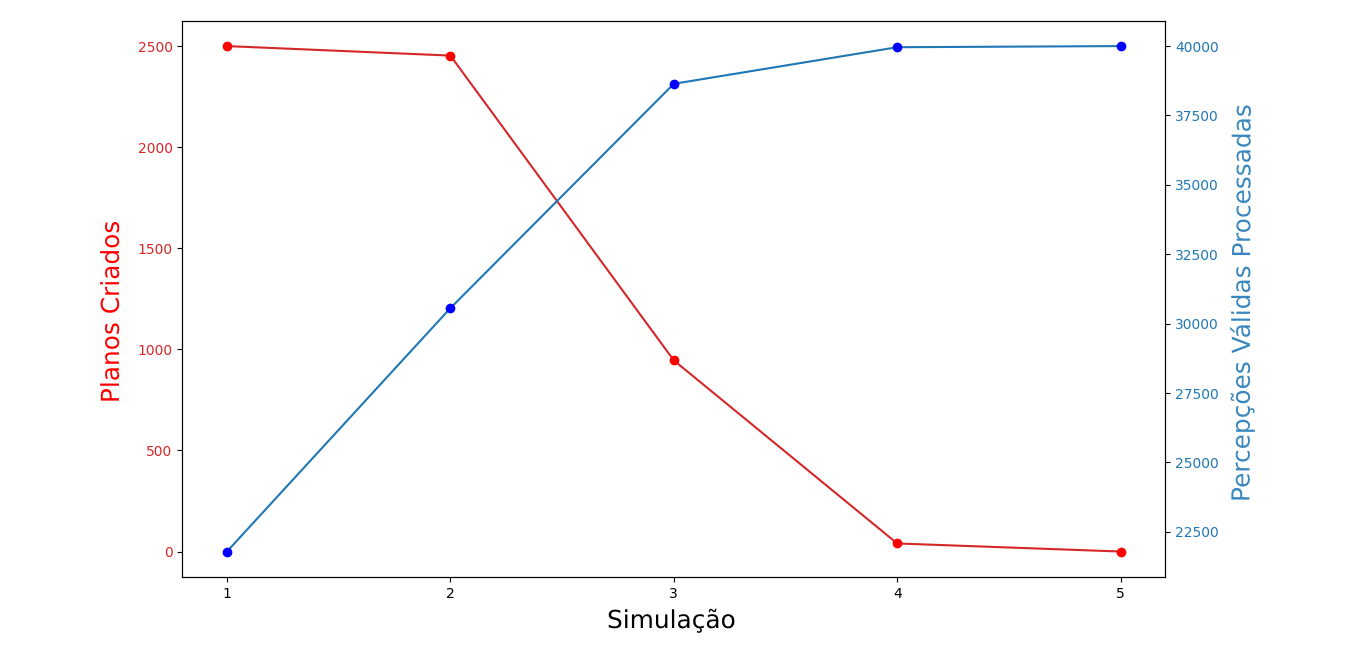
\includegraphics[width=\textwidth]{images/perceptions_vs_plans.png}
    \label{fig:perceptions_v_plans-experiment3}
    \caption{Evolução das percepções válidas processadas e dos planos novos criados ao longo das simulações.}
\end{figure}

